% Beamer deck: Diffusion Models -- From Adding Noise to Generating Images
% 12 content slides (+ 3 backup slides). Build: latexmk -pdf main.tex
% Speaker notes are kept in \note{...}; to print them instead of the slides, uncomment
%   \setbeameroption{show only notes}   (line below).
\documentclass[aspectratio=169,9pt,xcolor=table]{beamer}

\usepackage[T1]{fontenc}
\usepackage[utf8]{inputenc}
\usepackage{lmodern}
\usepackage{amsmath,amssymb,mathtools,booktabs,array,tabularx,pifont}
\usepackage{tikz}
\usetikzlibrary{arrows.meta,positioning,calc,fit}
\usepackage[skins]{tcolorbox}
\usepackage{appendixnumberbeamer}

% \setbeameroption{show only notes}   % uncomment to typeset the speaker notes only

%% ---------- colours (same palette as the report) ----------
\definecolor{hcmusblue}{HTML}{154A78}
\definecolor{fwd}{HTML}{247BA0}
\definecolor{rev}{HTML}{B96532}
\definecolor{ok}{HTML}{2E7D4F}
\definecolor{bad}{HTML}{B3372F}
\definecolor{muted}{HTML}{5A6572}
\definecolor{lightblue}{HTML}{EDF4FA}
\definecolor{lightgreen}{HTML}{EDF5F0}
\definecolor{lightorange}{HTML}{FFF3E7}

%% ---------- math shortcuts ----------
\newcommand{\E}{\mathbb{E}}
\newcommand{\R}{\mathbb{R}}
\newcommand{\Normal}{\mathcal{N}}
\newcommand{\Id}{\mathbf{I}}
\newcommand{\eps}{\varepsilon}
\newcommand{\ab}{\bar{\alpha}}
\DeclareMathOperator{\softmax}{softmax}
\DeclareMathOperator{\KL}{D_{KL}}

%% ---------- theme ----------
\usetheme{default}
\usefonttheme[onlymath]{serif}
\setbeamertemplate{navigation symbols}{}
\setbeamercolor{normal text}{fg=black!85}
\setbeamercolor{itemize item}{fg=hcmusblue}
\setbeamercolor{enumerate item}{fg=hcmusblue}
\setbeamertemplate{itemize item}{\small\raise0.1ex\hbox{$\blacktriangleright$}}
\setbeamertemplate{itemize subitem}{\footnotesize$\circ$}
\setbeamersize{text margin left=8mm,text margin right=8mm}
\setlength{\leftmargini}{1.1em}
\hyphenpenalty=5000 \exhyphenpenalty=5000 \tolerance=1500 \emergencystretch=2em
\setbeamertemplate{frametitle}{%
  \vskip 1.6mm
  {\color{rev}\fontsize{6}{7}\selectfont\bfseries\MakeUppercase{\insertframesubtitle}}\par
  \vskip -0.6mm
  {\color{hcmusblue}\fontsize{12.5}{14}\selectfont\bfseries\insertframetitle}\par
  \vskip 0.1mm
  {\color{hcmusblue!45}\rule{\textwidth}{0.4pt}}\par
  \vskip 0.6mm
}
\setbeamertemplate{footline}{%
  \leavevmode\hbox to\paperwidth{\hspace{8mm}%
    {\color{muted}\fontsize{6.5}{8}\selectfont CS420 \textperiodcentered{} Diffusion Models: From Adding Noise to Generating Images}%
    \hfill{\color{muted}\fontsize{6.5}{8}\selectfont\insertframenumber\,/\,\inserttotalframenumber}\hspace{8mm}}%
  \vskip 2.2mm}

%% ---------- boxes, tags, source line ----------
\tcbset{base/.style={enhanced,boxrule=0.5pt,arc=1.2mm,left=1.8mm,right=1.8mm,top=0.9mm,bottom=0.9mm,
  boxsep=0.3mm,fonttitle=\bfseries\footnotesize,toptitle=0.4mm,bottomtitle=0.4mm,lefttitle=1.8mm}}
\newtcolorbox{tbox}[3][]{base,colback=#3!5!white,colframe=#3,coltitle=white,title={#2},#1}
\newtcolorbox{nbox}[2][]{base,colback=#2!5!white,colframe=#2,#1}
\newcommand{\pill}[2]{{\setlength{\fboxsep}{1.2pt}\colorbox{#1}{\color{white}\fontsize{6}{7}\selectfont\bfseries\ #2\ }}}
\newcommand{\paper}{\pill{hcmusblue}{PAPER REPORTS}}
\newcommand{\ours}{\pill{rev}{OUR RUN}}
\newcommand{\oursum}{\pill{ok}{OUR EXAMPLE}}
\newcommand{\src}[1]{\par\vfill{\color{muted}\fontsize{6.2}{7.4}\selectfont #1\par}}
\usepackage{adjustbox}
\newcommand{\sech}[1]{{\color{hcmusblue}\small\bfseries #1}\par\vspace{-0.8mm}{\color{hcmusblue!45}\rule{\linewidth}{0.4pt}}\par\vspace{1.2mm}}
\newcolumntype{Y}{>{\raggedright\arraybackslash}X}
\newcommand{\yes}{\textcolor{ok}{\ding{51}}}
\newcommand{\no}{\textcolor{bad}{\ding{55}}}

\title{Diffusion Models: From Adding Noise to Generating Images}
\author{CS420 Seminar Team}
\date{}
\hypersetup{pdftitle={Diffusion Models: From Adding Noise to Generating Images},
  pdfauthor={HCMUS CS420 Seminar Team}}

\begin{document}

%% =====================================================================
%% 1. Title + guiding question  (~45 s)
%% =====================================================================
\begin{frame}[plain]
\begin{tikzpicture}[remember picture,overlay]
  \coordinate (NW) at (current page.north west);
  \fill[hcmusblue] (NW) rectangle ([yshift=-38mm]current page.north east);
  \node[anchor=north west,text=white,align=left,inner sep=0] at ([shift={(10mm,-6mm)}]NW)
    {{\fontsize{22}{26}\selectfont\bfseries Diffusion Models:}\\[1mm]
     {\fontsize{16}{19}\selectfont\bfseries From Adding Noise to Generating Images}};
  \node[anchor=north west,text=white!80!hcmusblue,inner sep=0] at ([shift={(10mm,-24mm)}]NW)
    {\fontsize{9}{11}\selectfont Understanding denoising-based generation through DDPM and LDM};
  \node[anchor=north west,text=white,inner sep=0] at ([shift={(10mm,-29.5mm)}]NW)
    {\fontsize{7.5}{9}\selectfont Cao Quang Hung (24125010) \quad Nguyen Trong Van Viet (24125023) \quad Huynh Chi Ton (24125020)};
  \node[anchor=north west,text=white!85!hcmusblue,inner sep=0] at ([shift={(10mm,-33.2mm)}]NW)
    {\fontsize{7.5}{9}\selectfont University of Science, VNU-HCM \quad\textperiodcentered\quad CS420 -- Artificial Intelligence};

  % guiding question
  \node[anchor=north west,draw=rev,line width=0.8pt,fill=lightorange,rounded corners=2mm,
        text width=82mm,inner sep=3mm,align=left] at ([shift={(10mm,-45mm)}]NW)
    {{\fontsize{7}{8}\selectfont\bfseries\color{rev}GUIDING QUESTION}\\[1.2mm]
     {\hyphenpenalty=10000\fontsize{13.5}{16.5}\selectfont\bfseries\color{hcmusblue}How can learning to remove noise enable a model to generate new images?}};

  % forward-noising strip
  \foreach \x/\xc/\t in {102/107.75/0,115/120.75/100,128/133.75/300,141/146.75/1000}{
    \node[anchor=north west,inner sep=0] at ([shift={(\x mm,-47mm)}]NW)
      {\includegraphics[width=11.5mm]{figures/state_\t.png}};
    \node[inner sep=0] at ([shift={(\xc mm,-61.5mm)}]NW)
      {\fontsize{6.5}{7}\selectfont\color{muted}$t=\t$};
  }
  \node[anchor=north west,inner sep=0,text=muted] at ([shift={(102mm,-43mm)}]NW)
    {\fontsize{6.5}{8}\selectfont forward noising: $x_0\to x_T$};

  % roadmap
  \foreach \x/\n/\col/\lab/\sub in {
      10/1/fwd/{Forward noising}/{DDPM \textperiodcentered{} Ho et al., 2020},
      46/2/rev/{Reverse denoising}/{DDPM \textperiodcentered{} noise prediction},
      82/3/ok/{Latent diffusion}/{LDM \textperiodcentered{} Rombach et al.},
      118/4/hcmusblue/{Evidence \& limits}/{our pretrained-model runs}}{
    \node[anchor=north west,fill=\col,text=white,rounded corners=1.5mm,minimum width=33mm,minimum height=12mm,
          inner sep=2mm,align=left,text width=29mm] at ([shift={(\x mm,-70mm)}]NW)
      {{\fontsize{8.5}{10}\selectfont\bfseries \n\ \lab}\\[-0.2mm]
       {\fontsize{6.5}{7.5}\selectfont \sub}};
  }
  \node[anchor=north west,text=muted,inner sep=0,text width=140mm] at ([shift={(10mm,-85mm)}]NW)
    {\fontsize{6.5}{8}\selectfont\textbf{Learning objective:} explain forward noising and reverse denoising, including why latent diffusion reduces computational demands.};
\end{tikzpicture}
\note{\textbf{(~45 s)} Hook: a denoiser repairs an image that exists; a generator must produce an image that never existed. What bridges the two? Introduce the guiding question and the four-part roadmap (it mirrors the learning objective).}
\end{frame}

%% =====================================================================
%% 2. Where diffusion fits  (~70 s)
%% =====================================================================
\begin{frame}
\frametitle{Where diffusion fits: three ways to generate images}
\framesubtitle{Positioning}
\begin{columns}[T,onlytextwidth]
\column{.31\textwidth}
\tcbset{before skip=0pt,after skip=1.2mm}
\sech{Generative vs.\ discriminative}
\begin{nbox}[fontupper=\scriptsize]{muted}
\textbf{Discriminative} learns $p(y\mid x)$: ``is this a cat?'' needs only class-separating features.
\end{nbox}
\begin{nbox}[fontupper=\scriptsize]{hcmusblue}
\textbf{Generative} learns $p(x)$ or $p(x\mid y)$: must capture shape, texture, lighting and layout.
\end{nbox}
\vspace{1mm}
\sech{Timeline}
{\scriptsize
{\color{rev}\textbf{2015}} diffusion framework (Sohl-Dickstein)\\[0.5mm]
{\color{rev}\textbf{2019}} score-based generation (Song \& Ermon)\\[0.5mm]
{\color{rev}\textbf{2020}} DDPM: predict the noise (Ho)\\[0.5mm]
{\color{rev}\textbf{2022}} LDM: latent space + cross-attention (Rombach)\par}
\column{.67\textwidth}
\sech{GAN vs.\ autoregressive vs.\ diffusion}
\centering
\adjustbox{width=\linewidth,trim={0 0 0 {.12\height}},clip}{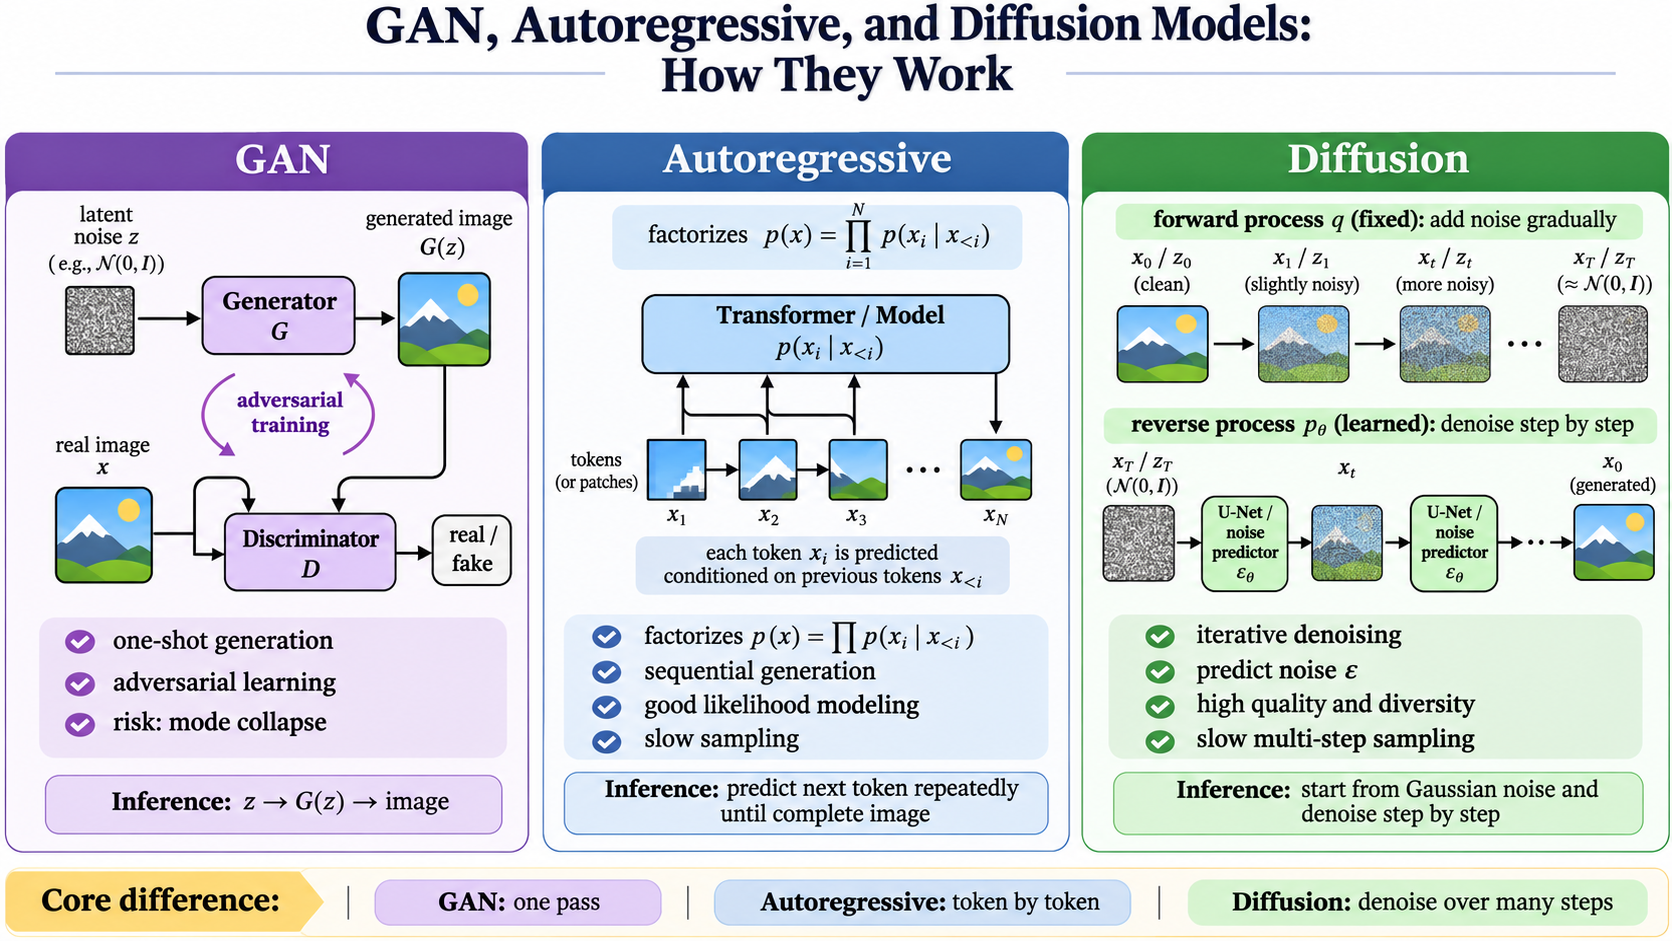
\includegraphics{figures/qualitative_comparison.png}}
\end{columns}
\src{Project illustration; sources: Goodfellow et al.\ 2014, van den Oord et al.\ 2016, Ho et al.\ 2020. Typical behaviour, not universal guarantees.}
\note{\textbf{(~70 s)} Walk the figure left to right: GAN = one pass but adversarial training; autoregressive = token by token; diffusion = denoise over many steps. Diffusion does not learn class boundaries; it learns the statistical structure of images by reversing a corruption we already know. Mention the cost: many sampling steps. Timeline: one sentence only.}
\end{frame}

%% =====================================================================
%% 3. Forward noising  (~90 s)
%% =====================================================================
\begin{frame}
\frametitle{Forward noising: a known way to destroy structure}
\framesubtitle{A \textperiodcentered{} Forward noising}
\begin{center}
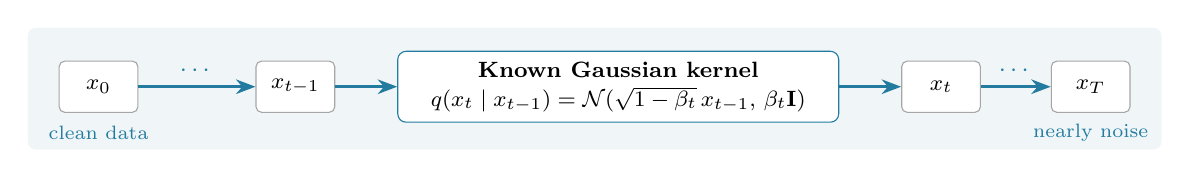
\begin{tikzpicture}[>=Stealth,font=\footnotesize,
  st/.style={draw=black!35,fill=white,rounded corners=2pt,minimum width=10mm,minimum height=6.5mm,inner sep=2pt},
  fl/.style={->,line width=0.9pt,fwd}]
  \fill[fwd!7,rounded corners=3pt] (0,-0.8) rectangle (14.4,0.75);
  \node[st] (x0) at (0.9,0) {$x_0$};
  \node[st] (xp) at (3.4,0) {$x_{t-1}$};
  \node[draw=fwd,fill=white,rounded corners=3pt,minimum width=5.6cm,minimum height=9mm,align=center,inner sep=3pt] (k) at (7.5,0)
    {\textbf{Known Gaussian kernel}\\[1pt]$q(x_t\mid x_{t-1})=\Normal(\sqrt{1-\beta_t}\,x_{t-1},\,\beta_t\Id)$};
  \node[st] (xt) at (11.6,0) {$x_t$};
  \node[st] (xT) at (13.5,0) {$x_T$};
  \draw[fl] (x0) -- node[above,font=\small]{$\cdots$} (xp);
  \draw[fl] (xp) -- (k);
  \draw[fl] (k) -- (xt);
  \draw[fl] (xt) -- node[above,font=\small]{$\cdots$} (xT);
  \node[font=\scriptsize,text=fwd] at (0.9,-0.58) {clean data};
  \node[font=\scriptsize,text=fwd] at (13.5,-0.58) {nearly noise};
\end{tikzpicture}
\end{center}
\vspace{-2mm}
\begin{columns}[T,onlytextwidth]
\column{.56\textwidth}
\begin{tbox}[fontupper=\small]{One step, and the jump to any $t$}{fwd}
\setlength{\abovedisplayskip}{2pt}\setlength{\belowdisplayskip}{2pt}
\[x_t=\sqrt{1-\beta_t}\,x_{t-1}+\sqrt{\beta_t}\,\eps,\quad \eps\sim\Normal(0,\Id)\]
\[\boxed{\,x_t=\sqrt{\ab_t}\,x_0+\sqrt{1-\ab_t}\,\eps\,}\]
\footnotesize $\beta_t\in(0,1)$ variance schedule, $\alpha_t=1-\beta_t$, $\ab_t=\prod_{j\le t}\alpha_j$. The index $t$ counts steps, not physical time.
\end{tbox}
\column{.42\textwidth}
\footnotesize
\begin{itemize}\setlength{\itemsep}{1.5pt}
\item $\beta_t$ both \emph{shrinks} the old signal ($\sqrt{1-\beta_t}$) and \emph{sets} the new noise level ($\sqrt{\beta_t}$).
\item $\Normal(0,\Id)$ is stationary, so after $T$ steps $x_T\approx\Normal(0,\Id)$: we know where generation will start.
\item DDPM schedule: $T=1000$, $\beta_t$ linear from $10^{-4}$ to $0.02$.
\end{itemize}
\end{columns}
\vspace{0.5mm}
\begin{nbox}[fontupper=\footnotesize]{rev}
\textbf{Why $T=1000$ small steps instead of one big step?}\quad
\textbf{(1)}~Small steps keep each \emph{reverse} step easy: nearly Gaussian, a small correction.\quad
\textbf{(2)}~Every noise level becomes a training task, from fine detail (small $t$) to coarse layout (large $t$) \emph{(our reading)}.
Training does not pay for $T$ steps (closed form); the cost appears at sampling $\rightarrow$ slide~6.
\end{nbox}
\src{Sohl-Dickstein et al.\ 2015; Ho et al.\ 2020 (notation $\alpha_t,\ab_t$). Diagram: original schematic.}
\note{\textbf{(~90 s)} The forward process is known and needs no learning: it hands us (noisy image, noise) pairs at every level. $t$ is a step index. Callout: one-step corruption is possible via the closed form, so training never simulates $T$ steps; the price of $T$ steps is paid at sampling.}
\end{frame}

%% =====================================================================
%% 4. Worked examples  (~80 s)
%% =====================================================================
\begin{frame}
\frametitle{Forward noising by hand and by eye}
\framesubtitle{A \textperiodcentered{} Forward noising}
\begin{columns}[T,onlytextwidth]
\column{.47\textwidth}
\begin{tbox}[fontupper=\footnotesize]{1-D calculation \oursum}{ok}
\setlength{\abovedisplayskip}{1pt}\setlength{\belowdisplayskip}{1pt}
$x_0=0.8,\ \beta_1=0.1,\ \eps=-0.5\ \Rightarrow\ \alpha_1=0.9$
\begin{align*}
\sqrt{\alpha_1}\,x_0&=\sqrt{0.9}\,(0.8)=0.758947\\
\sqrt{\beta_1}\,\eps&=\sqrt{0.1}\,(-0.5)=-0.158114\\
x_1&=\boxed{0.600833}
\end{align*}
\end{tbox}
\column{.51\textwidth}
\footnotesize
\begin{itemize}\setlength{\itemsep}{1pt}
\item $q(x_1\mid x_0{=}0.8)=\Normal(0.758947,\,0.1)$: mean $\sqrt{0.9}\,x_0$, standard deviation $\sqrt{0.1}=0.316$.
\item $\E[x_1\mid x_0]=\sqrt{0.9}\,x_0$ since $\E[\eps]=0$; the sample $0.6008$ differs because $\eps$ is one random draw.
\item $\beta_1=0.1$ only makes the arithmetic visible; the image below uses the small DDPM schedule.
\end{itemize}
\end{columns}
\vspace{1mm}
\begin{center}
\begin{tikzpicture}
  \node[inner sep=0] (img) {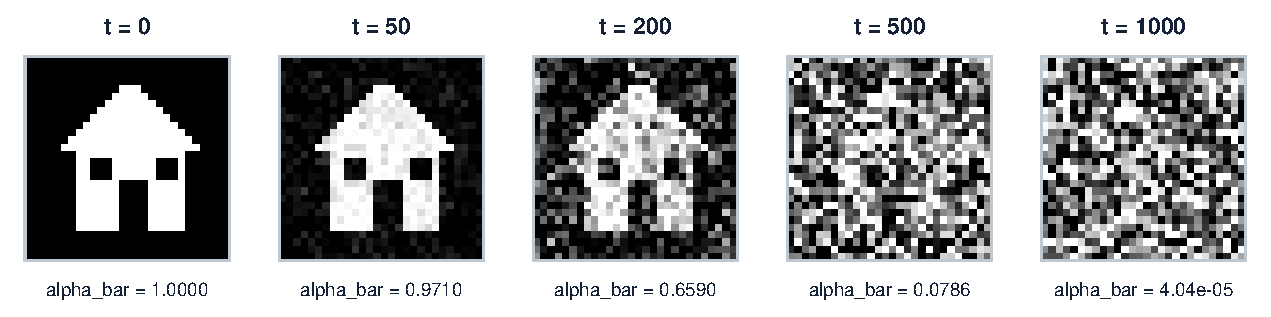
\includegraphics[width=9.4cm]{figures/noise_sequence.pdf}};
  \foreach \xx/\snr in {0.933/{SNR $=\infty$},2.791/{SNR $=33.5$},4.650/{SNR $=1.93$},6.508/{SNR $=0.085$},8.366/{SNR $\approx4\times10^{-5}$}}{
    \node[font=\scriptsize,text=hcmusblue,inner sep=1pt] at ($(img.south west)+(\xx cm,-1.8mm)$) {\snr};
  }
  \node[anchor=west,font=\scriptsize\bfseries,text=ok,align=left] at ($(img.east)+(0.2,0)$) {\oursum\\[2pt]28$\times$28\\house};
\end{tikzpicture}\\[0.5mm]
{\footnotesize $\mathrm{SNR}=\ab_t/(1-\ab_t)$: the house is clearly visible at $t=50$, noise dominates at $t=500$, almost nothing is left at $t=T$.}
\end{center}
\src{Our example (no model): synthetic house, $T=1000$, linear $\beta_t$ from $10^{-4}$ to $0.02$, one sampled trajectory.}
\note{\textbf{(~80 s)} Walk the arithmetic aloud: 0.7589 - 0.1581 = 0.6008. Stress that the expectation is sqrt(0.9) x0, the realization differs. Then the image: house visible at t=50 (SNR 33.5), gone at t=500 (SNR below 0.1). The two examples use different betas on purpose.}
\end{frame}

%% =====================================================================
%% 5. Reverse denoising  (~90 s)
%% =====================================================================
\begin{frame}
\frametitle{Reverse denoising: learn to undo one small step}
\framesubtitle{B \textperiodcentered{} Reverse denoising}
\begin{center}
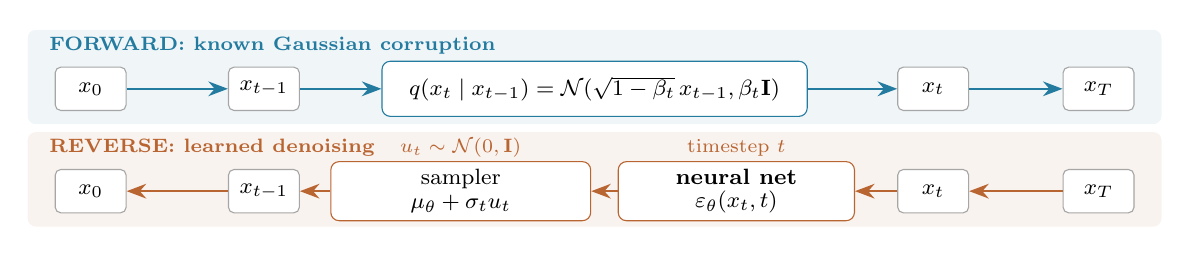
\begin{tikzpicture}[>=Stealth,font=\footnotesize,
  st/.style={draw=black!35,fill=white,rounded corners=2pt,minimum width=9mm,minimum height=5.5mm,inner sep=2pt},
  opf/.style={draw=fwd,fill=white,rounded corners=3pt,minimum height=7mm,align=center,inner sep=3pt},
  opr/.style={draw=rev,fill=white,rounded corners=3pt,minimum height=7.5mm,align=center,inner sep=2pt}]
  % forward band
  \fill[fwd!7,rounded corners=3pt] (0,1.3) rectangle (14.4,2.5);
  \node[anchor=west,font=\scriptsize\bfseries,text=fwd] at (0.15,2.3) {FORWARD: known Gaussian corruption};
  \node[st] (fx0) at (0.8,1.75) {$x_0$};
  \node[st] (fxp) at (3.0,1.75) {$x_{t-1}$};
  \node[opf,minimum width=5.4cm] (fk) at (7.2,1.75) {$q(x_t\mid x_{t-1})=\Normal(\sqrt{1-\beta_t}\,x_{t-1},\beta_t\Id)$};
  \node[st] (fxt) at (11.5,1.75) {$x_t$};
  \node[st] (fxT) at (13.6,1.75) {$x_T$};
  \foreach \a/\b in {fx0/fxp,fxp/fk,fk/fxt,fxt/fxT}{\draw[->,line width=0.9pt,fwd] (\a) -- (\b);}
  % reverse band
  \fill[rev!8,rounded corners=3pt] (0,0) rectangle (14.4,1.2);
  \node[anchor=west,font=\scriptsize\bfseries,text=rev] at (0.15,1.0) {REVERSE: learned denoising};
  \node[st] (rx0) at (0.8,0.45) {$x_0$};
  \node[st] (rxp) at (3.0,0.45) {$x_{t-1}$};
  \node[opr,minimum width=3.3cm] (rs) at (5.5,0.45) {sampler\\[-1pt]$\mu_\theta+\sigma_t u_t$};
  \node[opr,minimum width=3.0cm] (rn) at (9.0,0.45) {\textbf{neural net}\\[-1pt]$\eps_\theta(x_t,t)$};
  \node[st] (rxt) at (11.5,0.45) {$x_t$};
  \node[st] (rxT) at (13.6,0.45) {$x_T$};
  \foreach \a/\b in {rxT/rxt,rxt/rn,rn/rs,rs/rxp,rxp/rx0}{\draw[->,line width=0.9pt,rev] (\a) -- (\b);}
  \node[font=\scriptsize,text=rev] at (5.5,1.0) {$u_t\sim\Normal(0,\Id)$};
  \node[font=\scriptsize,text=rev] at (9.0,1.0) {timestep $t$};
\end{tikzpicture}
\end{center}
\vspace{-2.5mm}
\begin{columns}[T,onlytextwidth]
\column{.49\textwidth}
\begin{tbox}[fontupper=\footnotesize]{One reverse step}{rev}
\setlength{\abovedisplayskip}{1pt}\setlength{\belowdisplayskip}{1pt}
$p_\theta(x_{t-1}\mid x_t)=\Normal\big(\mu_\theta(x_t,t),\sigma_t^2\Id\big)$
\[\mu_\theta=\frac{1}{\sqrt{\alpha_t}}\Big(x_t-\frac{\beta_t}{\sqrt{1-\ab_t}}\,\boldsymbol{\eps_\theta(x_t,t)}\Big)\]
\emph{Why predict $\eps$, not $x_0$?} $\eps\sim\Normal(0,\Id)$ is a simple, normalized target; it also encodes the score, $-\eps_\theta/\sqrt{1-\ab_t}\approx\nabla\log q_t(x_t)$.
\end{tbox}
\column{.49\textwidth}
\begin{tbox}[fontupper=\footnotesize]{Training objective}{hcmusblue}
\setlength{\abovedisplayskip}{1pt}\setlength{\belowdisplayskip}{1pt}
\[L_{\text{simple}}=\E_{t,x_0,\eps}\big[\|\eps-\eps_\theta(x_t,t)\|^2\big]\]
\begin{enumerate}\setlength{\itemsep}{0pt}
\item draw image $x_0$, $t\sim\mathrm{U}\{1..T\}$, $\eps\sim\Normal(0,\Id)$
\item build $x_t=\sqrt{\ab_t}\,x_0+\sqrt{1-\ab_t}\,\eps$
\item predict $\eps_\theta(x_t,t)$; gradient step on the error
\end{enumerate}
\paper\ CIFAR-10 FID $3.17$ vs.\ $13.51$ (variational)
\end{tbox}
\end{columns}
\src{Diagram: original schematic after Sohl-Dickstein et al.\ 2015 and Ho et al.\ 2020. $L_{\text{simple}}$ is a reweighted surrogate of the variational bound (Ho et al.\ 2020, Tables 1--2).}
\note{\textbf{(~90 s)} Central figure: blue = known, orange = learned. The network never sees the clean image at inference. Training in 3 lines. Why epsilon: normalized target and link to score; derivation (KL, posterior mean) goes to Q\&A.}
\end{frame}

%% =====================================================================
%% 6. From denoising to generation  (~110 s)
%% =====================================================================
\begin{frame}
\frametitle{From denoising to generation: answering the guiding question}
\framesubtitle{B \textperiodcentered{} Reverse denoising}
\begin{columns}[T,onlytextwidth]
\column{.52\textwidth}
\begin{tbox}[fontupper=\footnotesize]{Sampling: no real image needed}{rev}
\textbf{1.}~$x_T\sim\Normal(0,\Id)$ \quad(fresh noise)\\
\textbf{2.}~for $t=T,\dots,1$:\; $x_{t-1}=\mu_\theta(x_t,t)+\sigma_t\,u_t$,\; $u_t\sim\Normal(0,\Id)$\\
\textbf{3.}~return $x_0$ \quad(no noise is added at $t=1$)
\end{tbox}
\vspace{1mm}
{\footnotesize\textbf{Why removing noise generates new images}
\begin{enumerate}\setlength{\itemsep}{1pt}
\item \textbf{Free supervision:} the forward process gives $(x_t,\eps)$ pairs at every noise level.
\item \textbf{Shared structure:} to predict the noise, the network must learn what images have in common.
\item \textbf{Small stochastic steps:} each step is a gentle correction; fresh $u_t$ makes every seed a different image.
\end{enumerate}}
\vspace{0.5mm}
\begin{nbox}[fontupper=\footnotesize]{bad}
\textbf{Why not one step?} Training $x_T\mapsto x_0$ with squared error gives $\E[x_0\mid x_T]\approx\E[x_0]$ because $x_T$ carries almost no information about $x_0$: the average, blurry image. Small \emph{forward} steps are what make small \emph{reverse} steps possible.
\end{nbox}
\column{.46\textwidth}
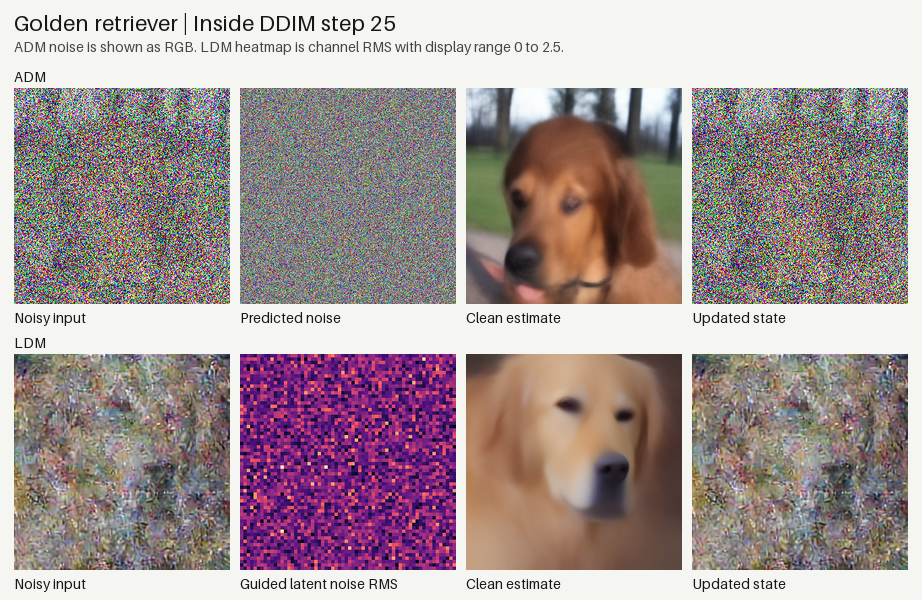
\includegraphics[width=\linewidth]{figures/retriever_step25.png}\\[-0.5mm]
{\footnotesize \ours\ \emph{Inside DDIM update 25, golden retriever.} Top: pixel ADM; bottom: latent LDM.}
\vspace{0.5mm}
\footnotesize
\begin{itemize}\setlength{\itemsep}{1pt}
\item The \emph{clean estimate} already shows head and muzzle, while the \emph{updated state} is still noisy.
\item A forward pass from the final image makes the retriever's features vanish gradually (cf.\ slide~4).
\end{itemize}
\end{columns}
\src{Our run: OpenAI ADM (pixel), CompVis cin256-v2 (latent), ImageNet, 50 DDIM steps; one sample per class. Sampling: Ho et al.\ 2020, Alg.~2.}
\note{\textbf{(~110 s)} This slide answers the guiding question: free supervision, shared structure, small stochastic steps. One-step training collapses to the mean image. The picture shows the mechanism: at step 25 the clean estimate already has a dog, the state still looks like noise.}
\end{frame}

%% =====================================================================
%% 7. Autoencoder  (~80 s)
%% =====================================================================
\begin{frame}
\frametitle{Inside the autoencoder: how images become latents}
\framesubtitle{C \textperiodcentered{} Latent diffusion}
\begin{center}
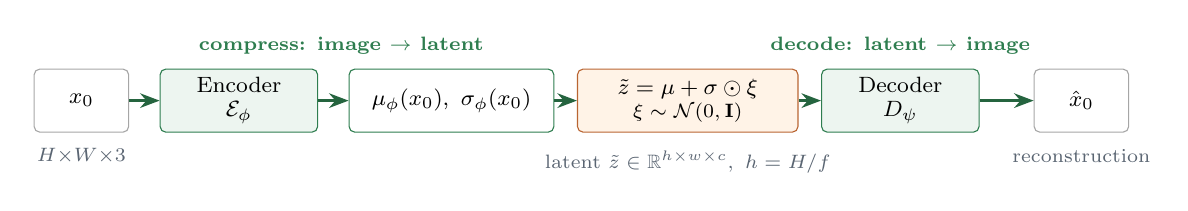
\begin{tikzpicture}[>=Stealth,font=\footnotesize,
  box/.style={draw=ok,fill=lightgreen,rounded corners=2pt,minimum height=8mm,inner sep=3pt,align=center},
  io/.style={draw=black!35,fill=white,rounded corners=2pt,minimum height=8mm,minimum width=12mm,inner sep=2pt,align=center},
  fl/.style={->,line width=0.9pt,ok!80!black}]
  \node[io] (x) at (0.7,0) {$x_0$};
  \node[box,minimum width=2.0cm] (enc) at (2.7,0) {Encoder\\[-1pt]$\mathcal E_\phi$};
  \node[box,fill=white,minimum width=2.6cm] (par) at (5.4,0) {$\mu_\phi(x_0),\ \sigma_\phi(x_0)$};
  \node[box,draw=rev,fill=lightorange,minimum width=2.8cm] (smp) at (8.4,0) {$\tilde z=\mu+\sigma\odot\xi$\\[-1pt]\scriptsize$\xi\sim\Normal(0,\Id)$};
  \node[box,minimum width=2.0cm] (dec) at (11.1,0) {Decoder\\[-1pt]$D_\psi$};
  \node[io] (xh) at (13.4,0) {$\hat x_0$};
  \foreach \a/\b in {x/enc,enc/par,par/smp,smp/dec,dec/xh}{\draw[fl] (\a) -- (\b);}
  \node[font=\scriptsize,text=muted] at (0.7,-0.7) {$H{\times}W{\times}3$};
  \node[font=\scriptsize,text=muted] at (8.4,-0.78) {latent $\tilde z\in\R^{h\times w\times c},\ h=H/f$};
  \node[font=\scriptsize,text=muted] at (13.4,-0.7) {reconstruction};
  \node[font=\scriptsize\bfseries,text=ok] at (4.0,0.7) {compress: image $\to$ latent};
  \node[font=\scriptsize\bfseries,text=ok] at (11.1,0.7) {decode: latent $\to$ image};
\end{tikzpicture}
\end{center}
\vspace{-2.5mm}
\begin{columns}[T,onlytextwidth]
\column{.325\textwidth}
\begin{tbox}[fontupper=\footnotesize,height=3.75cm]{VAE objective}{hcmusblue}
\setlength{\abovedisplayskip}{1pt}\setlength{\belowdisplayskip}{1pt}
\textbf{Reconstruction} + \textbf{KL to the prior}:
\[\begin{gathered}\E[-\log p_\psi(x_0\mid\tilde z)]\\+\KL\big(q_\phi\|\Normal(0,\Id)\big)\end{gathered}\]
The decoder must rebuild the image; the KL keeps codes near $\Normal(0,\Id)$. \textbf{Problem:} pixel-wise squared error averages plausible details, so images turn \emph{blurry}.
\end{tbox}
\column{.325\textwidth}
\begin{tbox}[fontupper=\footnotesize,height=3.75cm]{LDM: a perceptual compressor}{ok}
\textbf{1.}~\emph{Perceptual loss}: compare deep features, so the result must \emph{look} like the input.\\
\textbf{2.}~\emph{Patch-based adversarial loss}: a discriminator judges local patches $\Rightarrow$ realistic texture.\\
\textbf{3.}~\emph{Light regularizer}: weak KL (\textbf{KL-reg}) or a codebook in the decoder (\textbf{VQ-reg}).\\
{\scriptsize Ours: Churches = KL, $f{=}8$; ImageNet = VQ, $f{=}4$.}
\end{tbox}
\column{.325\textwidth}
\begin{tbox}[fontupper=\footnotesize,height=3.75cm]{What changes for diffusion}{rev}
$\bullet$ Latent keeps its 2-D layout, so a U-Net can process it.\\
$\bullet$ Autoencoder: trained once, then \textbf{frozen}.\\
$\bullet$ Diffusion learns the \emph{distribution of latents}; clean latents are not $\Normal(0,\Id)$, so decoding $\tilde z\sim\Normal(0,\Id)$ is not enough.\\
$\bullet$ Encoder noise $\xi\neq$ diffusion noise $\eps_z$.
\end{tbox}
\end{columns}
\src{Kingma \& Welling 2014; Rombach et al.\ 2022, Sec.~3.1; Zhang et al.\ 2018; Isola et al.\ 2017; Esser et al.\ 2021; van den Oord et al.\ 2017.}
\note{\textbf{(~80 s)} The autoencoder is the learned compression step. VAE in one line: encoder outputs a distribution, decoder reconstructs, KL regularizes. Pixel MSE gives blur, so LDM uses perceptual + adversarial loss. Key points: frozen after stage 1; diffusion replaces the VAE prior; do not confuse xi with epsilon\_z.}
\end{frame}

%% =====================================================================
%% 8. Why latent diffusion is cheaper + pipeline  (~90 s)
%% =====================================================================
\begin{frame}
\frametitle{Why latent diffusion is cheaper: same loop, smaller state}
\framesubtitle{C \textperiodcentered{} Latent diffusion}
\begin{center}
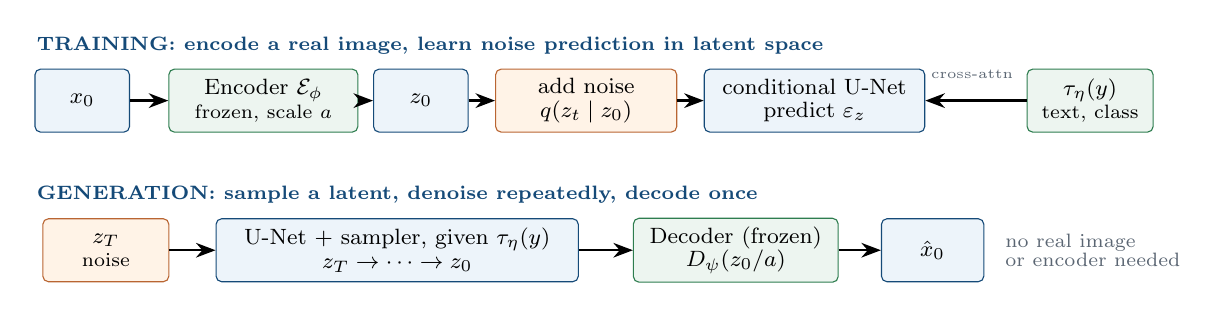
\begin{tikzpicture}[>=Stealth,font=\footnotesize,
  box/.style={draw=hcmusblue,fill=lightblue,rounded corners=2pt,minimum height=8mm,inner sep=3pt,align=center},
  frz/.style={draw=ok,fill=lightgreen,rounded corners=2pt,minimum height=8mm,inner sep=3pt,align=center},
  nz/.style={draw=rev,fill=lightorange,rounded corners=2pt,minimum height=8mm,inner sep=3pt,align=center},
  fl/.style={->,line width=0.9pt}]
  \node[anchor=west,font=\scriptsize\bfseries,text=hcmusblue] at (0,3.15) {TRAINING: encode a real image, learn noise prediction in latent space};
  \node[box,minimum width=1.2cm] (x) at (0.7,2.45) {$x_0$};
  \node[frz,minimum width=2.4cm] (e) at (3.0,2.45) {Encoder $\mathcal E_\phi$\\[-1pt]\scriptsize frozen, scale $a$};
  \node[box,minimum width=1.2cm] (z) at (5.0,2.45) {$z_0$};
  \node[nz,minimum width=2.3cm] (n) at (7.1,2.45) {add noise\\[-1pt]$q(z_t\mid z_0)$};
  \node[box,minimum width=2.8cm] (u) at (10.0,2.45) {conditional U-Net\\[-1pt]predict $\eps_z$};
  \node[frz,minimum width=1.6cm] (c) at (13.5,2.45) {$\tau_\eta(y)$\\[-1pt]\scriptsize text, class};
  \draw[fl] (x)--(e); \draw[fl] (e)--(z); \draw[fl] (z)--(n); \draw[fl] (n)--(u);
  \draw[fl] (c)--(u);
  \node[font=\tiny,text=muted] at (12.0,2.78) {cross-attn};
  \node[anchor=west,font=\scriptsize\bfseries,text=hcmusblue] at (0,1.25) {GENERATION: sample a latent, denoise repeatedly, decode once};
  \node[nz,minimum width=1.6cm] (zT) at (1.0,0.55) {$z_T$\\[-1pt]\scriptsize noise};
  \node[box,minimum width=4.6cm] (s) at (4.7,0.55) {U-Net + sampler, given $\tau_\eta(y)$\\[-1pt]$z_T\to\cdots\to z_0$};
  \node[frz,minimum width=2.6cm] (d) at (9.0,0.55) {Decoder (frozen)\\[-1pt]$D_\psi(z_0/a)$};
  \node[box,minimum width=1.3cm] (xo) at (11.5,0.55) {$\hat x_0$};
  \node[anchor=west,font=\scriptsize,text=muted,align=left] at (12.3,0.55) {no real image\\[-1pt]or encoder needed};
  \draw[fl] (zT)--(s); \draw[fl] (s)--(d); \draw[fl] (d)--(xo);
\end{tikzpicture}
\end{center}
\vspace{-2.5mm}
\begin{columns}[T,onlytextwidth]
\column{.49\textwidth}
\begin{tbox}[fontupper=\footnotesize]{Smaller state per denoising step}{ok}
\begin{itemize}\setlength{\itemsep}{1.5pt}
\item $f{=}4$: $256{\times}256{\times}3\to64{\times}64{\times}3$, i.e.\ \textbf{16$\times$ fewer spatial positions}. \paper\ Table~8
\item LSUN Churches (KL-8): $196{,}608$ vs.\ $4{,}096$ values, \textbf{$\approx$48$\times$ fewer}. \oursum\ (arithmetic from run settings)
\end{itemize}
\end{tbox}
\column{.49\textwidth}
\begin{tbox}[fontupper=\footnotesize]{Same principle, new space}{hcmusblue}
\setlength{\abovedisplayskip}{1pt}\setlength{\belowdisplayskip}{1pt}
\[L_{\text{LDM}}=\E\big[\|\eps_z-\eps_\theta(z_t,t,\tau_\eta(y))\|^2\big]\]
Forward noising and $\eps$-prediction are unchanged; DDIM adds fewer steps on top. \textbf{Caveat:} compression caps quality (fine text, small objects), and runtime/memory depend on more than state size $\rightarrow$ slide~10.
\end{tbox}
\end{columns}
\src{Pipeline: original schematic after Rombach et al.\ 2022, Fig.~3 and Secs.~3.1--3.3; sampler: Song et al.\ 2021 (DDIM).}
\note{\textbf{(~90 s)} Direct answer to the learning objective: the loop (predict noise, step) is identical, but each U-Net call works on a latent that is 16x (paper) or about 48x (our churches run) smaller; decode once at the end. Warn: a smaller state does not automatically mean lower peak memory; see slide 10.}
\end{frame}

%% =====================================================================
%% 9. Cross-attention + prompt control  (~100 s)
%% =====================================================================
\begin{frame}
\frametitle{Cross-attention: steering the denoiser with a prompt}
\framesubtitle{C \textperiodcentered{} Latent diffusion}
\begin{columns}[T,onlytextwidth]
\column{.47\textwidth}
\begin{tbox}[fontupper=\footnotesize]{Prompt $\to$ tokens $\to$ attention}{ok}
\setlength{\abovedisplayskip}{1.5pt}\setlength{\belowdisplayskip}{1.5pt}
$C=\tau_\eta(y)$ (frozen CLIP text encoder in Stable Diffusion v1.4)
\[Q=FW_Q,\quad K=CW_K,\quad V=CW_V\]
\[O=\softmax\big(QK^{\top}/\sqrt{d}\big)\,V\]
\textbf{Queries come from the image; keys and values come from the condition.} A region turning into a bus can draw on the tokens \emph{red} and \emph{bus}.
\end{tbox}
\vspace{0.5mm}
\footnotesize
\begin{itemize}\setlength{\itemsep}{1pt}
\item Recomputed at every layer and step: the prompt steers each denoising prediction; it is \emph{not} pasted onto the final image.
\item Only $\tau_\eta$ changes with the modality: text, class label (1 token, our ImageNet LDM), layout; maps and masks are concatenated with $z_t$.
\item Classifier-free guidance $\eps_u+s(\eps_c-\eps_u)$: larger $s$, closer to the prompt, less diverse.
\end{itemize}
\column{.51\textwidth}
{\footnotesize \ours\ \textbf{Stable Diffusion v1.4, seed 2027, same initial latent}}\\[1mm]
\setlength{\tabcolsep}{1.5pt}
\begin{tabular}{@{}p{2.2cm}p{2.2cm}p{2.2cm}@{}}
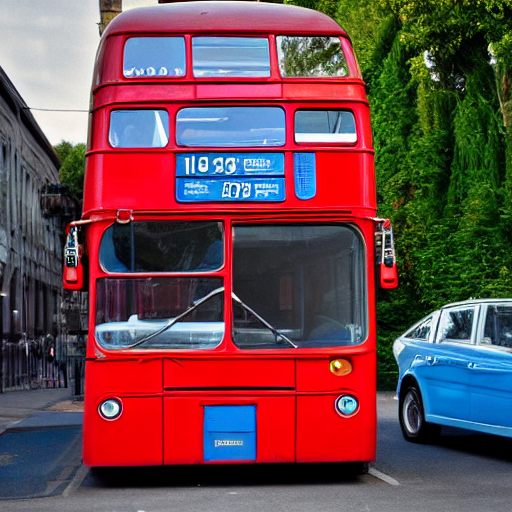
\includegraphics[width=2.2cm]{figures/prompt/2027_reference.png} &
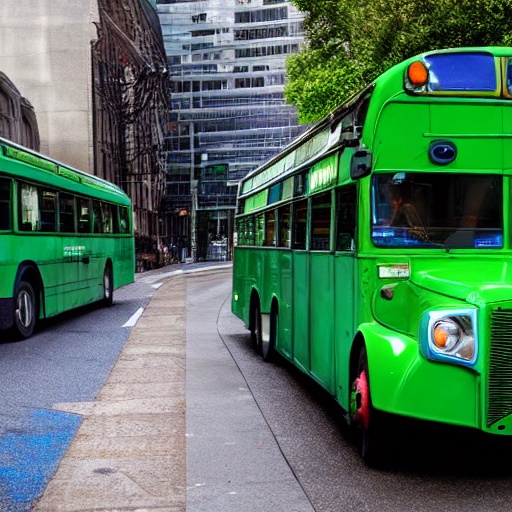
\includegraphics[width=2.2cm]{figures/prompt/2027_change_color.png} &
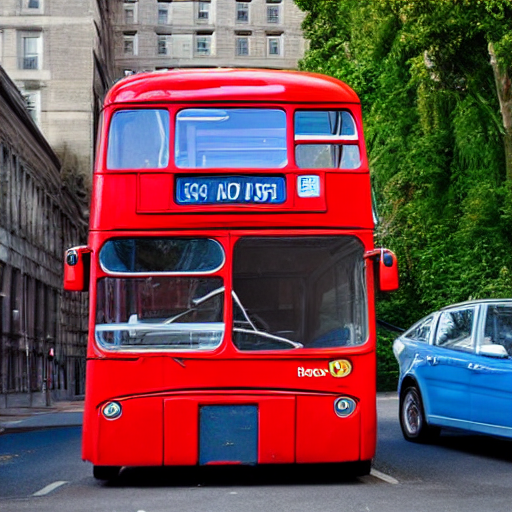
\includegraphics[width=2.2cm]{figures/prompt/2027_change_side.png}\\[-0.5mm]
\raggedright\scriptsize\textbf{Reference}\newline\tiny``a red bus to the left of a blue car'' &
\raggedright\scriptsize\textbf{red $\to$ green}\newline\tiny``a green bus to the left of a blue car'' &
\raggedright\scriptsize\textbf{left $\to$ right}\newline\tiny``a red bus to the right of a blue car''
\end{tabular}\\[1mm]
\footnotesize
\begin{itemize}\setlength{\itemsep}{1pt}
\item Colour edit: green bus at \textbf{all 4 seeds} \yes, but no clear blue car; seed 2027 shows two green buses \no.
\item Side edit: no clear left-to-right swap; the red bus stays on the left \no.
\item Cross-attention is \emph{soft}: attributes can bind to the wrong object, or a token can be ignored.
\end{itemize}
\end{columns}
\src{Vaswani et al.\ 2017; Rombach et al.\ 2022, Sec.~3.3; Ho \& Salimans 2022; Radford et al.\ 2021; Chefer et al.\ 2023. Images: our run, CFG 7.5, 50 DDIM steps; 16 images checked by eye, an illustration and not a general conclusion.}
\note{\textbf{(~100 s)} Mechanism first (queries from the image, keys/values from the text), then the evidence: colour changes succeed, object identity and left/right do not. Cross-attention is soft; CFG does not guarantee counting or spatial relations. Be explicit: 16 images, visual check only.}
\end{frame}

%% =====================================================================
%% 10. Pixel vs latent on LSUN Churches  (~80 s)
%% =====================================================================
\begin{frame}
\frametitle{Pixel vs.\ latent diffusion on LSUN Churches}
\framesubtitle{D \textperiodcentered{} Evidence and limits}
{\footnotesize \ours\ Pretrained checkpoints (no training by us) \textperiodcentered{} Tesla T4 \textperiodcentered{} batch 1 \textperiodcentered{} 50 DDIM steps ($\eta=0$) \textperiodcentered{} 4 seeds (2026--2029) \textperiodcentered{} warm-up excluded, GPU-synchronized timing\par}
\vspace{1mm}
\begin{columns}[T,onlytextwidth]
\column{.52\textwidth}
{\footnotesize
\renewcommand{\arraystretch}{1.3}
\begin{tabularx}{\linewidth}{@{}>{\bfseries}p{2.9cm}YY@{}}
\toprule
\rowcolor{hcmusblue!12}Criterion & Pixel DDPM & LDM-KL-8\\
\midrule
Denoising state & $256{\times}256{\times}3$ & $32{\times}32{\times}4$\\
Median latency (s/img) & 6.10 & \textbf{2.44} ($2.5\times$ faster)\\
Peak CUDA alloc.\ (GiB) & \textbf{0.75} & 1.68\\
\bottomrule
\end{tabularx}}
\vspace{1.5mm}
\begin{nbox}[fontupper=\footnotesize]{hcmusblue}
\paper\ Rombach et al., Table 6 (Places inpainting, $256^2$): pixel LDM-1 vs.\ latent LDM-4 $=0.26\to0.97$ samples/s; FID@2k $24.74\to15.21$.
\end{nbox}
\column{.46\textwidth}
\centering
\setlength{\tabcolsep}{1pt}
\begin{tabular}{@{}rcccc@{}}
 & \scriptsize 2026 & \scriptsize 2027 & \scriptsize 2028 & \scriptsize 2029\\
\raisebox{4mm}{\scriptsize DDPM} &
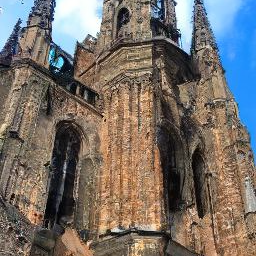
\includegraphics[width=1.4cm]{figures/churches/ddpm_2026.png} &
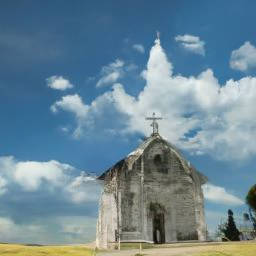
\includegraphics[width=1.4cm]{figures/churches/ddpm_2027.png} &
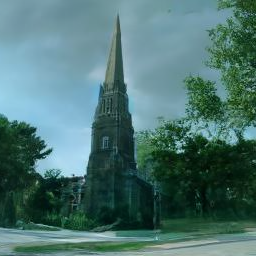
\includegraphics[width=1.4cm]{figures/churches/ddpm_2028.png} &
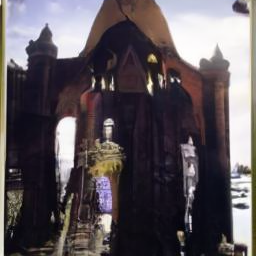
\includegraphics[width=1.4cm]{figures/churches/ddpm_2029.png}\\
\raisebox{4mm}{\scriptsize LDM} &
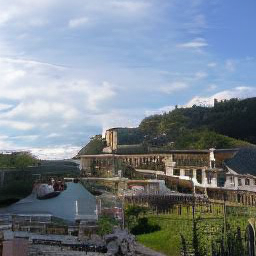
\includegraphics[width=1.4cm]{figures/churches/ldm_2026.png} &
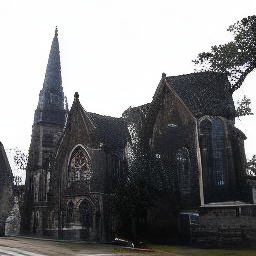
\includegraphics[width=1.4cm]{figures/churches/ldm_2027.png} &
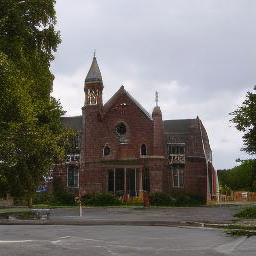
\includegraphics[width=1.4cm]{figures/churches/ldm_2028.png} &
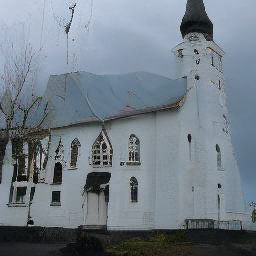
\includegraphics[width=1.4cm]{figures/churches/ldm_2029.png}
\end{tabular}\\[0.5mm]
{\scriptsize\raggedright Pixel: clear steeple (2028), dark 2029 hides detail. Latent: clear facades (2027--2029), 2026 is a distant complex. Each model draws noise in its own state space.\par}
\end{columns}
\vspace{1.5mm}
\begin{nbox}[fontupper=\footnotesize]{rev}
\textbf{Takeaway:} the latent model was faster but used \emph{more} peak memory in our setup, so ``cheaper compute'' is not ``cheaper in every resource''. Four images per model, one checkpoint pair, no FID: an illustration, not a benchmark.
\end{nbox}
\src{Our run: ddpm-ema-church-256 vs.\ CompVis LDM-KL-8 (FP32); latency includes the decoder. Paper values: Rombach et al.\ 2022, Table 6.}
\note{\textbf{(~80 s)} Read the table, then the caveat. If asked why LDM peak memory is higher: we only measured it; the two checkpoints differ in architecture/decoder, an untested hypothesis. Paper numbers are for a different task (inpainting), shown only as external evidence.}
\end{frame}

%% =====================================================================
%% 11. Limitations  (~50 s)
%% =====================================================================
\begin{frame}
\frametitle{Limitations: training data, copyright and bias}
\framesubtitle{D \textperiodcentered{} Evidence and limits}
\begin{columns}[T,onlytextwidth]
\column{.325\textwidth}
\begin{tbox}[fontupper=\small,height=4.0cm]{1. Training data}{hcmusblue}
\emph{A model only knows what its data contains.}
\begin{itemize}\setlength{\itemsep}{1.5pt}
\item Church checkpoints specialize in churches.
\item ImageNet conditioning uses a fixed class vocabulary.
\item Text models inherit the attributes and relations present in captions.
\end{itemize}
\end{tbox}
\column{.325\textwidth}
\begin{tbox}[fontupper=\small,height=4.0cm]{2. Bias}{rev}
Bianchi et al.\ (2023): ordinary prompts to text-to-image systems can yield \textbf{demographic stereotypes} at scale.

\vspace{1.5mm}
\textbf{Our bus-and-car demo does not measure bias.}
\end{tbox}
\column{.325\textwidth}
\begin{tbox}[fontupper=\small,height=4.0cm]{3. Copyright and memorization}{bad}
\begin{itemize}\setlength{\itemsep}{1.5pt}
\item Carlini et al.\ (2023) extracted \textbf{memorized training images} from diffusion models.
\item Data provenance matters for copyright; the U.S.\ Copyright Office (2025) analyses training under \emph{U.S.\ law}, not Vietnamese law.
\item This does not mean every generated image is a copy.
\end{itemize}
\end{tbox}
\end{columns}
\vspace{1.5mm}
\begin{nbox}[fontupper=\footnotesize]{muted}
\textbf{Method limits:} many sampling steps \textperiodcentered{} quality capped by autoencoder reconstruction \textperiodcentered{} soft cross-attention (slide~9) \textperiodcentered{} our experiments are small illustrations (no FID, no bias metrics), not benchmarks.
\end{nbox}
\src{Bianchi et al.\ 2023; Carlini et al.\ 2023; U.S.\ Copyright Office 2025, Copyright and AI, Part 3 (pre-publication version).}
\note{\textbf{(~50 s)} Critical analysis: say plainly what our experiments do not prove. The legal source is a US policy analysis, not a conclusion about every generated image, and not Vietnamese law.}
\end{frame}

%% =====================================================================
%% 12. Conclusion  (~45 s)
%% =====================================================================
\begin{frame}
\frametitle{Conclusion: answering the guiding question}
\framesubtitle{Take-home}
\begin{nbox}[colframe=rev,colback=lightorange,fontupper=\small]{rev}
\textbf{How can learning to remove noise enable a model to generate new images?}\\[1mm]
Because the forward process gives \textbf{free training pairs at every noise level}, a network trained to predict the noise learns \textbf{shared image structure}, and running it from \textbf{fresh noise in many small stochastic steps} turns noise into a new sample.
\end{nbox}
\vspace{1.5mm}
\begin{columns}[T,onlytextwidth]
\column{.325\textwidth}
\begin{tbox}[fontupper=\footnotesize,height=2.5cm]{1. Forward noising}{fwd}
Known Gaussian chain with schedule $\beta_t$; the closed form $x_t=\sqrt{\ab_t}\,x_0+\sqrt{1-\ab_t}\,\eps$ reaches any $t$ directly.
\end{tbox}
\column{.325\textwidth}
\begin{tbox}[fontupper=\footnotesize,height=2.5cm]{2. Reverse denoising}{rev}
Learn $p_\theta(x_{t-1}\mid x_t)$ by predicting the noise ($L_{\text{simple}}$); sample by iterating small steps from $\Normal(0,\Id)$.
\end{tbox}
\column{.325\textwidth}
\begin{tbox}[fontupper=\footnotesize,height=2.5cm]{3. Latent diffusion}{ok}
Same principle on autoencoder latents: cheaper steps ($\approx2.5\times$ faster in our run; $0.26\to0.97$ samples/s in the paper) and prompts via cross-attention. Costs: reconstruction limit, memory not necessarily lower.
\end{tbox}
\end{columns}
\vspace{0.5mm}
\begin{center}
{\small\itshape Capability is bounded by the training data, and by what we actually measured.}\\[1.5mm]
{\large\bfseries\color{hcmusblue}Thank you \textperiodcentered{} Questions?}\\[0.5mm]{\scriptsize\color{muted}References and figure sources: backup slides}
\end{center}
\note{\textbf{(~45 s)} Close the loop on the guiding question in one sentence; the three recap cards mirror the learning objective. Hand over to Q\&A; every member answers at least one question.}
\end{frame}

%% =====================================================================
%% Backup slides (not counted in the 12 content slides)
%% =====================================================================
\appendix
\setbeamertemplate{footline}{%
  \leavevmode\hbox to\paperwidth{\hspace{8mm}%
    {\color{muted}\fontsize{6.5}{8}\selectfont CS420 \textperiodcentered{} Diffusion Models: From Adding Noise to Generating Images}%
    \hfill{\color{muted}\fontsize{6.5}{8}\selectfont Backup}\hspace{8mm}}%
  \vskip 2.2mm}

\newcommand{\refitem}[1]{\par\noindent\hangindent=1.2em\hangafter=1 \textbullet\ #1\par\vspace{1pt}}

\begin{frame}
\frametitle{References (1/2)}
\framesubtitle{Backup}
\fontsize{7}{8.4}\selectfont
\begin{columns}[T,onlytextwidth]
\column{.49\textwidth}
\refitem{J.~Ho, A.~Jain, P.~Abbeel. Denoising Diffusion Probabilistic Models. \emph{NeurIPS}, 2020.}
\refitem{R.~Rombach, A.~Blattmann, D.~Lorenz, P.~Esser, B.~Ommer. High-Resolution Image Synthesis with Latent Diffusion Models. \emph{CVPR}, 2022.}
\refitem{J.~Sohl-Dickstein, E.~Weiss, N.~Maheswaranathan, S.~Ganguli. Deep Unsupervised Learning using Nonequilibrium Thermodynamics. \emph{ICML}, 2015.}
\refitem{Y.~Song, S.~Ermon. Generative Modeling by Estimating Gradients of the Data Distribution. \emph{NeurIPS}, 2019.}
\refitem{J.~Song, C.~Meng, S.~Ermon. Denoising Diffusion Implicit Models. \emph{ICLR}, 2021.}
\refitem{D.~P.~Kingma, M.~Welling. Auto-Encoding Variational Bayes. \emph{ICLR}, 2014.}
\column{.49\textwidth}
\refitem{I.~Goodfellow et al. Generative Adversarial Nets. \emph{NeurIPS}, 2014.}
\refitem{A.~van den Oord, N.~Kalchbrenner, K.~Kavukcuoglu. Pixel Recurrent Neural Networks. \emph{ICML}, 2016.}
\refitem{A.~van den Oord, O.~Vinyals, K.~Kavukcuoglu. Neural Discrete Representation Learning. \emph{NeurIPS}, 2017.}
\refitem{P.~Esser, R.~Rombach, B.~Ommer. Taming Transformers for High-Resolution Image Synthesis. \emph{CVPR}, 2021.}
\refitem{R.~Zhang et al. The Unreasonable Effectiveness of Deep Features as a Perceptual Metric. \emph{CVPR}, 2018.}
\refitem{P.~Isola, J.-Y.~Zhu, T.~Zhou, A.~A.~Efros. Image-to-Image Translation with Conditional Adversarial Networks. \emph{CVPR}, 2017.}
\end{columns}
\end{frame}

\begin{frame}
\frametitle{References (2/2) and figure sources}
\framesubtitle{Backup}
\fontsize{7}{8.4}\selectfont
\begin{columns}[T,onlytextwidth]
\column{.49\textwidth}
\refitem{A.~Vaswani et al. Attention Is All You Need. \emph{NeurIPS}, 2017.}
\refitem{J.~Ho, T.~Salimans. Classifier-Free Diffusion Guidance. arXiv:2207.12598, 2022.}
\refitem{A.~Radford et al. Learning Transferable Visual Models From Natural Language Supervision (CLIP). \emph{ICML}, 2021.}
\refitem{H.~Chefer et al. Attend-and-Excite: Attention-Based Semantic Guidance for Text-to-Image Diffusion Models. \emph{ACM TOG}, 2023.}
\column{.49\textwidth}
\refitem{R.~Rombach, P.~Esser. Stable Diffusion v1.4 Model Card (CompVis). Hugging Face, 2022.}
\refitem{F.~Bianchi et al. Easily Accessible Text-to-Image Generation Amplifies Demographic Stereotypes at Large Scale. \emph{FAccT}, 2023.}
\refitem{N.~Carlini et al. Extracting Training Data from Diffusion Models. \emph{USENIX Security}, 2023.}
\refitem{U.S.~Copyright Office. Copyright and Artificial Intelligence, Part 3: Generative AI Training (pre-publication version), 2025. A U.S.\ policy analysis, not a statement of Vietnamese law.}
\end{columns}
\vspace{2mm}
\begin{nbox}[fontupper=\fontsize{7}{8.4}\selectfont]{muted}
\textbf{Figures and results.} The schematics (slides 3, 5, 7, 8) are original drawings of the cited methods. The 1-D calculation, the 28$\times$28 noising sequence, the LSUN Churches timing, the ImageNet denoising traces and the Stable Diffusion prompt test are our own runs with pretrained checkpoints (no training by us); published numbers are attributed to Ho et al.\ 2020 and Rombach et al.\ 2022.\\[1mm]
\textbf{AI assistance.} OpenAI Codex (report drafting, code, checks); Claude (slide drafting and Beamer preparation).
\end{nbox}
\end{frame}

\end{document}
